\documentclass[a4paper, 14pt]{extarticle}
\usepackage[russian]{babel}
\usepackage[T1]{fontenc}
\usepackage{fontspec}
\usepackage{indentfirst}
\usepackage{enumitem}
\usepackage{graphicx}
\usepackage[
  left=20mm,
  right=10mm,
  top=20mm,
  bottom=20mm
]{geometry}
\usepackage{parskip}
\usepackage{titlesec}
\usepackage{xurl}
\usepackage{hyperref}
\usepackage{float}
\usepackage[
  figurename=Рисунок,
  labelsep=endash,
]{caption}
\usepackage[outputdir=build, newfloat]{minted}

\hypersetup{
  colorlinks=true,
  linkcolor=black,
  filecolor=blue,
  urlcolor=blue,
}

\renewcommand*{\labelitemi}{---}
\setmainfont{Times New Roman}
\setmonofont{JetBrains Mono}[
  SizeFeatures={Size=11},
]

\newenvironment{code}{\captionsetup{type=listing}}{}
\SetupFloatingEnvironment{listing}{name=Листинг}

\setminted{
  fontsize=\footnotesize,
  frame=lines,
  framesep=2mm,
}

\setlength{\parskip}{6pt}

\setlength{\parindent}{1cm}
\setlist[itemize]{itemsep=0em,topsep=0em,parsep=0em,partopsep=0em,leftmargin=2.0cm,wide}
\setlist[enumerate]{itemsep=0em,topsep=0em,parsep=0em,partopsep=0em,leftmargin=2.0cm,wide}

\renewcommand{\thesection}{\arabic{section}.}
\renewcommand{\thesubsection}{\thesection\arabic{subsection}.}
\renewcommand{\thesubsubsection}{\thesubsection\arabic{subsubsection}.}

\titleformat{\section}{\normalfont\bfseries}{\thesection}{0.5em}{}
\titleformat{\subsection}{\normalfont\bfseries}{\thesubsection}{0.5em}{}

\titleformat*{\section}{\normalfont\bfseries}
\titleformat*{\subsection}{\normalfont\bfseries}

\linespread{1.5}
\renewcommand{\baselinestretch}{1.5}

\begin{document}

\begin{titlepage}
  \vspace{0pt plus2fill}
  \noindent

  \vspace{0pt plus6fill}
  \begin{center}
    Санкт-Петербургский национальный исследовательский университет
    информационных технологий, механики и оптики

    \vspace{0pt plus3fill}

    Факультет инфокоммуникационных технологий

    Направление подготовки 11.03.02

    \vspace{0pt plus2fill}

    Лабораторная работа №3
  \end{center}

  \vspace{0pt plus6fill}
  \begin{flushright}
    Выполнил: \\
    Швалов Даниил Андреевич

    Группа: К33211

    Проверила: \\
    Марченко Елена Вадимовна
  \end{flushright}

  \vspace{0pt plus5fill}
  \begin{center}
    Санкт-Петербург

    2024
  \end{center}
\end{titlepage}

\section{Введение}

\textbf{Цель работы}:
\begin{itemize}
  \item модифицировать существующее приложение на
  \foreignlanguage{english}{Delphi}, чтобы оно отвечало заданным требованиям;
  \item разработать клиент-серверное приложение.
\end{itemize}

\section{Ход работы}

\subsection*{
  Задание №1. Модификация примера обработки документов Word в Delphi
}

В данном задании необходимо модифицировать исходный код существующей программы
на \foreignlanguage{english}{Delphi}. Изначально данная программа добавляет
текст в документ так, как это ожидается. Однако, при каждом добавлении нового
текста программа открывает новое окно \foreignlanguage{english}{Word}.
Необходимо сделать так, чтобы текст добавлялся в уже открытое окно.

Для этого в существующую функцию <<\foreignlanguage{english}{BitBtn3Click}>>
была добавлена проверка на количество открытых документов. Если количество равно
нулю, то открывается новый документ. Если это не так, то ничего не происходит,
используется уже существующий документ. Исходный код полученной функции показан
на рисунке \ref{fig:task-1-1}.

\begin{figure}[H]
  \centering
  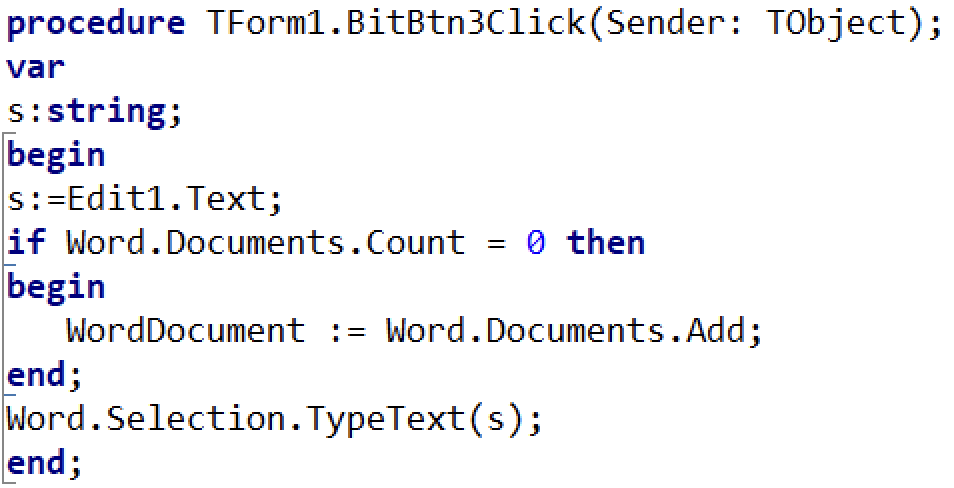
\includegraphics[width=0.6\textwidth]{images/task-1/1.png}
  \caption{Исходный код функции <<\foreignlanguage{english}{BitBtn3Click}>>}
  \label{fig:task-1-1}
\end{figure}

Также была создана функция-обработчик для кнопки <<Сохранить в файл>>, которая
была автоматически названа <<\foreignlanguage{english}{BitBtn4Click}>>. В нее
был добавлен код, который сохраняет открытый
\foreignlanguage{english}{Word}-файл по пути, введенному в текстовое поле.
Исходный код данной функции представлен на рисунке \ref{fig:task-1-2}.

\begin{figure}[H]
  \centering
  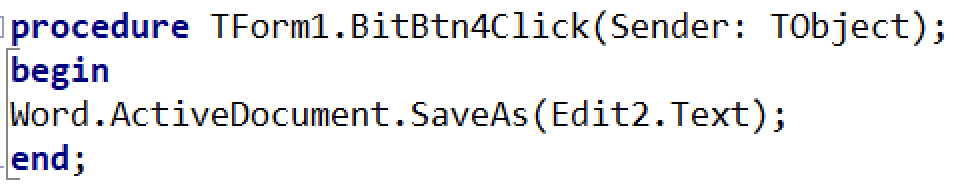
\includegraphics[width=0.6\textwidth]{images/task-1/2.png}
  \caption{Исходный код функции <<\foreignlanguage{english}{BitBtn4Click}>>}
  \label{fig:task-1-2}
\end{figure}

После добавления необходимого кода приложение было скомпилировано и запущено. На
рисунке \ref{fig:task-1-3} продемонстрирован пример работы программы: в файл
было добавлено две одинаковых строки. Тем самым, было показано, что требуемая
функциональность была поддержана в приложении.

\begin{figure}[H]
  \centering
  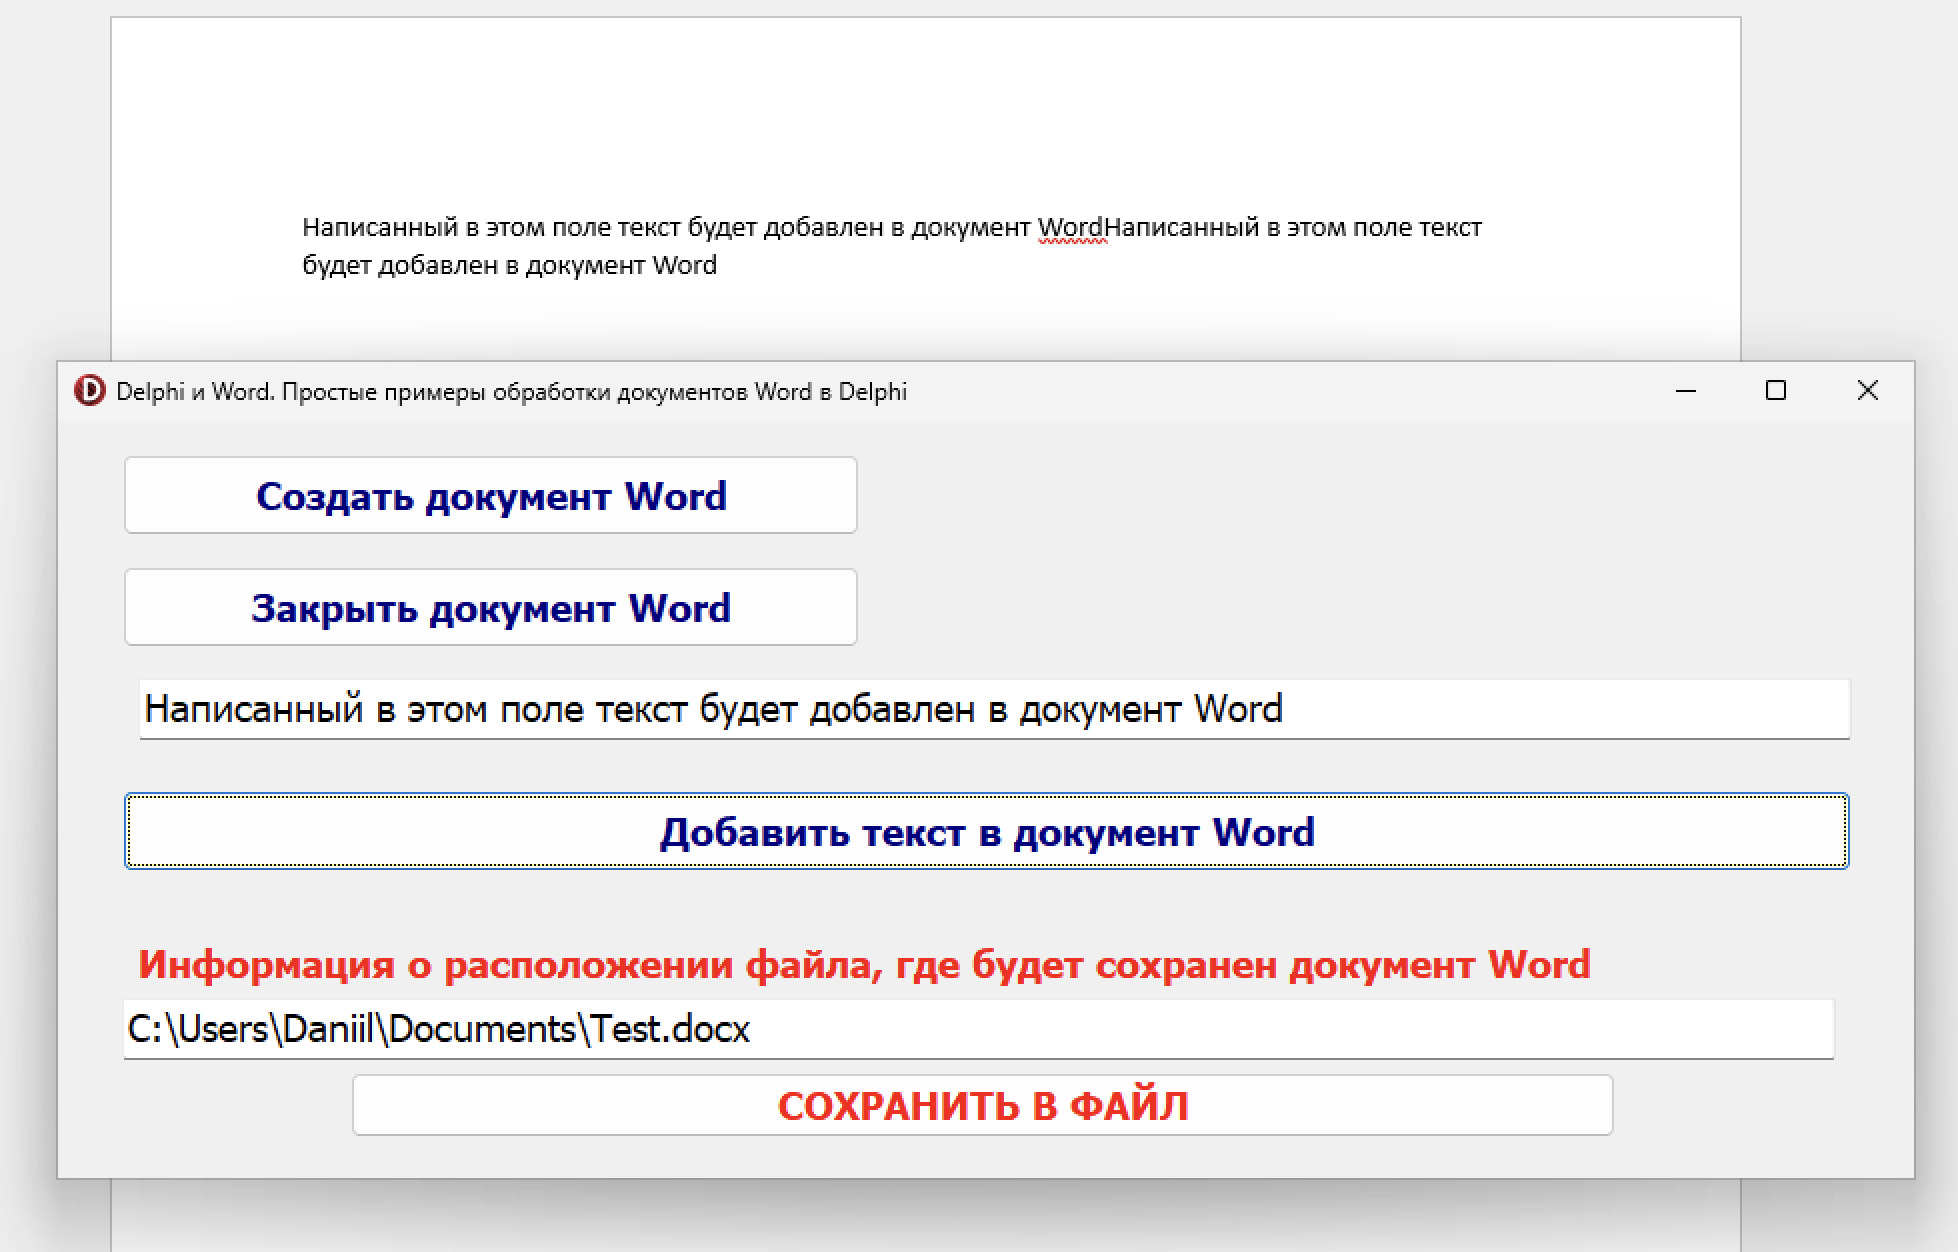
\includegraphics[width=\textwidth]{images/task-1/3.png}
  \caption{Пример работы программы}
  \label{fig:task-1-3}
\end{figure}

\subsection*{Задание №2. Разработка клиент-серверного приложения}

В данном задании необходимо разработать клиент-серверное приложение, которое по
заданным точкам прямой находит ее коэффициенты и точки аппроксимированной
прямой.

Для реализации приложения был выбран язык программирования C++, поскольку он
позволяет создавать высокопроизводительные приложения, при этом обладает большим
количеством библиотек. Для реализации серверной части была выбрана библиотека
\foreignlanguage{english}{Boost Beast}, а для реализации клиентского интерфейса
--- библиотека \foreignlanguage{english}{Qt Framework}.

При открытии приложения пользователя встречает окно, показанное на рисунке
\ref{fig:task-2-1}. В нем пользователю предлагается ввести точки прямой. С
помощью кнопки <<+>> пользователь может добавлять новые точки, а с помощью
кнопки <<->> удалять.

\begin{figure}[H]
  \centering
  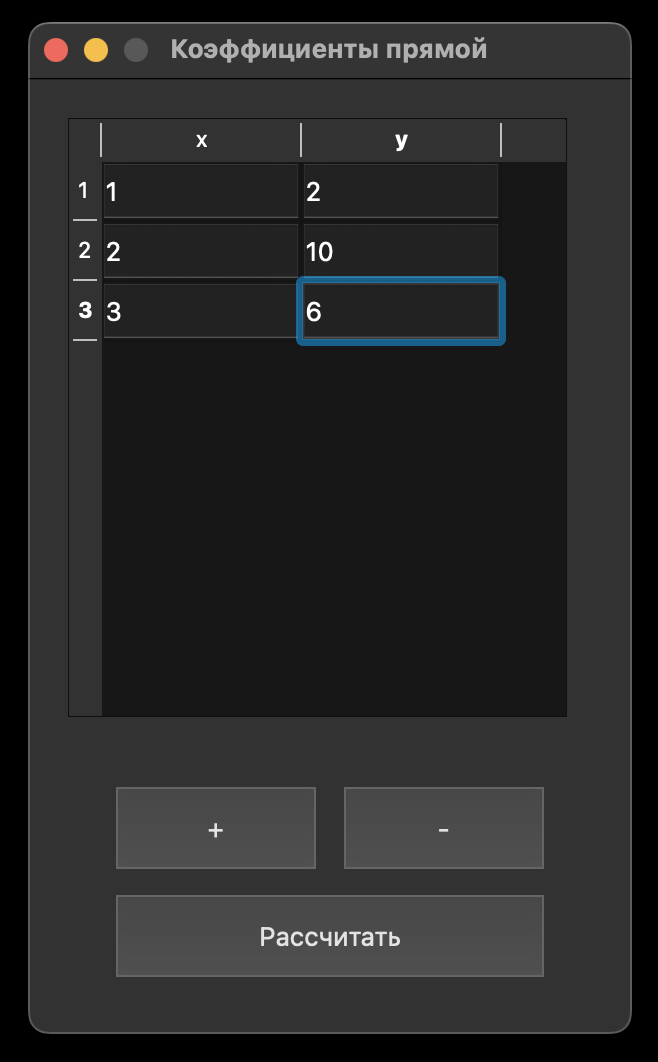
\includegraphics[width=0.4\textwidth]{images/task-2/1.png}
  \caption{Окно ввода коэффициентов}
  \label{fig:task-2-1}
\end{figure}

При нажатии на кнопку <<Рассчитать>> открывается новое окно, показанное на
рисунке \ref{fig:task-2-2}. В нем отображаются коэффициенты прямой \(a\), \(b\)
и \(R\), а также точки аппроксимированной прямой.

При нажатии на кнопку <<Рассчитать>> клиент отправляет запрос на сервер, в
котором содержится информация о точках. После этого сервер начинает обрабатывать
полученные данные, а затем отправляет ответ клиенту с информацией о
коэффициентах и рассчитанных точках. Именно это информация и отображается в
новой таблице.

\begin{figure}[H]
  \centering
  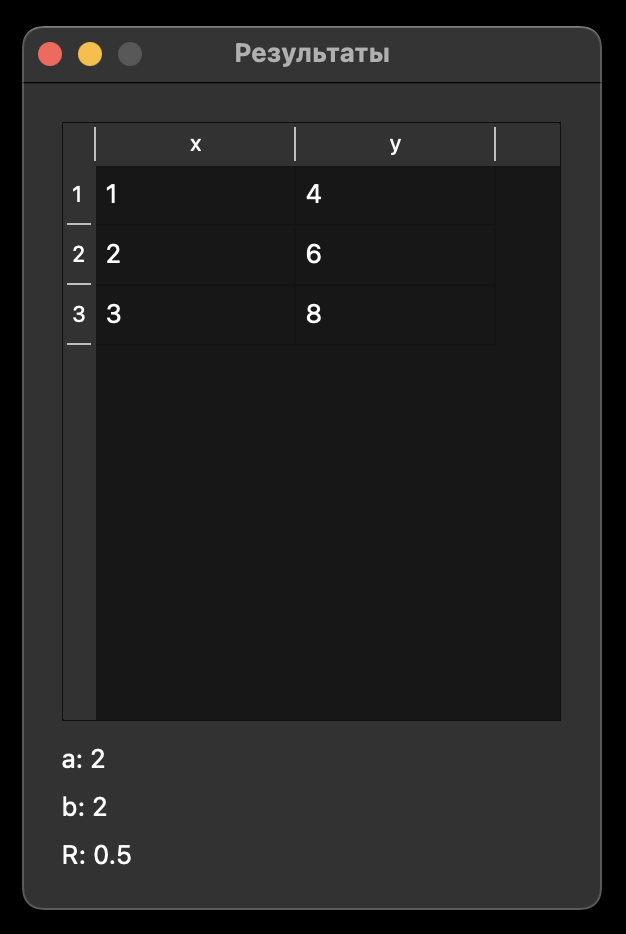
\includegraphics[width=0.4\textwidth]{images/task-2/2.png}
  \caption{Окно с результатами}
  \label{fig:task-2-2}
\end{figure}

\section{Вывод}

В данной лабораторной работе была произведена доработка приложения на
\foreignlanguage{english}{Delphi}, которое добавляет текст в документ
\foreignlanguage{english}{Word}. После доработки приложение стало более
дружелюбным для пользователя, поскольку теперь оно позволяет добавлять не одну
строку в документ, а сколько угодно.

Также в данной лабораторной работе было разработано клиент-серверное приложение
для вычисления коэффициентов прямой по заданным точкам. Благодаря данному
приложению пользователям нет необходимости считать коэффициенты руками: теперь
достаточно ввести полученные точки в программу. Основным преимуществом данной
программы является то, что все расчеты происходят на сервере, а не на клиенте.
Благодаря этому расчеты можно проводить быстрее.

Цель, поставленная в начале работы, достигнута, задачи выполнены.

\end{document}
